\chapter{Background}
\label{cha:bkg}
%Literature Review
This chapter provides the readers with detailed biology background of object recognition in the brain and the fundamental principles of neural modelling using spiking neural networks.
This is followed by an introduction to the neuromorphic hardware platform specialised for neural simulations of visual processing.

\section{How the Brain Represent Objects?}
\label{sec:bio}

\begin{figure}
	\centering
	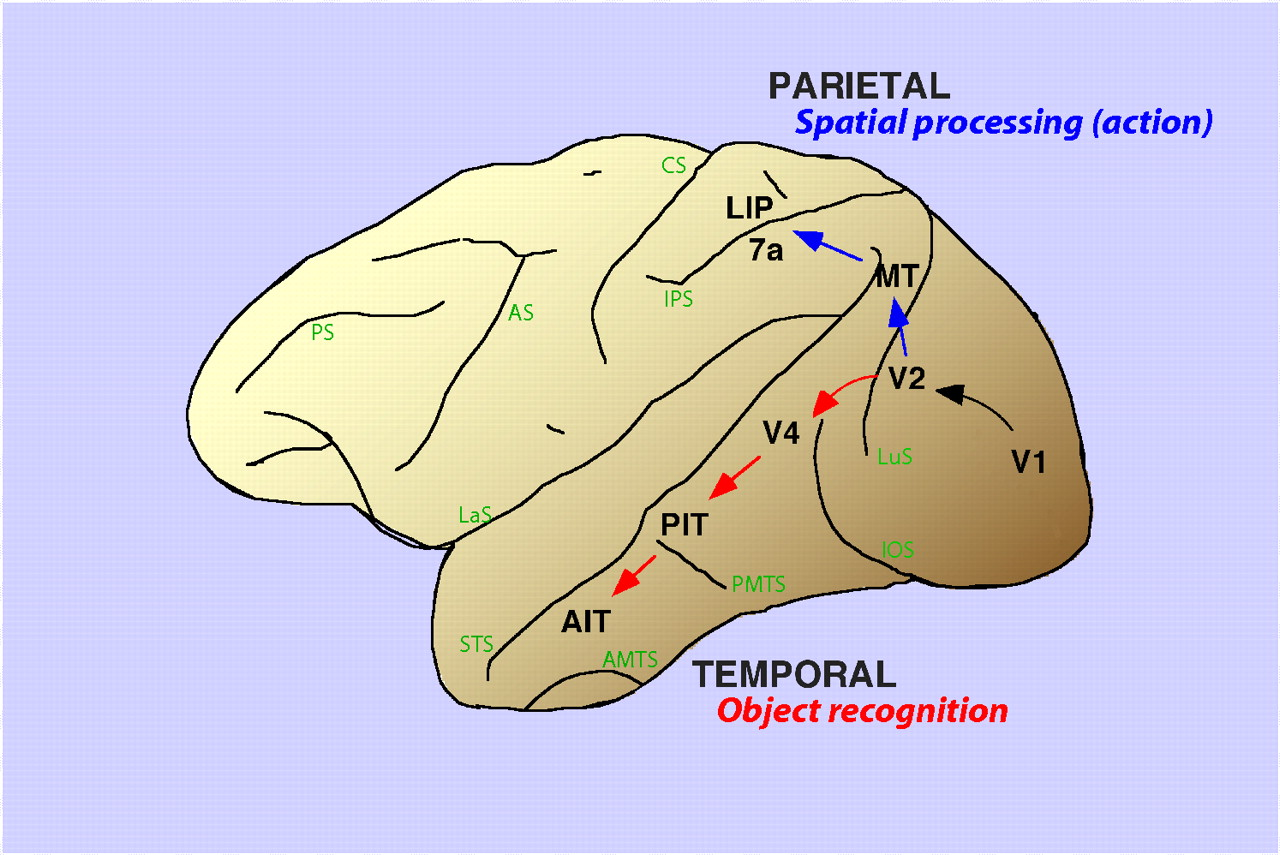
\includegraphics[width=0.8\textwidth]{pics/twoPaths.jpg}
	\caption{The dorsal and ventral pathway in the brain~\cite{lehky2007comparison}.
	The dorsal stream (blue) arrives to the parietal lobe, whereas the ventral pathway (red) reaches the inferotemporal (IT) cortex in the temporal lobe.}
	\label{Fig:TwoPath}
\end{figure}
The central visual system consists of several cortical areas responsible for visual processing, which are placed in a hierarchical pattern according to the anatomical experiments~\cite{felleman1991distributed}.
There are two basic streams locating in the visual area: a dorsal and a ventral pathway (Figure~\ref{Fig:TwoPath}).

They differ in behavioural patterns according to the observation from brain lesions~\cite{prado2005two}, and also in functions where the dorsal pathway targets on the `where' tasks and the ventral on the `what'.
The ventral visual stream holds the critical circuits for object recognition and stimulus identification, whereas the dorsal pathway pathway contributes to the processing of the spatial location of the stimulus~\cite{prado2005two, Ungerleider1994157}.
Another definition of the difference between these two pathways is a `perception/action' dichotomy: the ventral (`perception') stream perceives the world by means of object recognition and memory, while the dorsal (`action') stream provides real-time visual guidance for motor actions such as eye movements and grasping objects~\cite{goodale1992separate}. 

This research mainly focuses on the ventral visual pathway, since it dominates the object recognition among the cortical areas.
Thus, the dorsal pathway will beyond the scope of the this study. 


\subsection{Cortical Areas in The Ventral Visual Pathway}
The ventral visual pathway starts from the primary visual cortex V1 in the occipital cortex through areas such as V2 and V4 to the Inferotemporal (IT) cortex.
These cortex areas are divided based on the anatomical experiments and retinotopic maps.
Accordingly, the IT complex is commonly parsed into sub areas such as TEO and TE~\cite{janssen2000selectivity,von1947neocortex} or posterior IT (PIT), central IT (CIT), and anterior IT (AIT)~\cite{felleman1991distributed}.
\subsubsection{Primary Visual Cortex:V1}
As the simplest and earliest cortical area in the ventral stream, the primary visual cortex V1 is the best-studied since the well-known discovery of the orientation selectivity by Hubel and Wiesel~\cite{hubel1959receptive} in 1958.
The retinotopic map is well-defined to transform spatial information from retinal image to V1~\cite{tootell1982deoxyglucose}.
In human and animals with a fovea in the retina, the central 10 degrees of the visual field occupies roughly half of V1.
This distorted retinotopic map in V1 is a phenomenon known as cortical magnification.

\begin{figure}
	\centering
	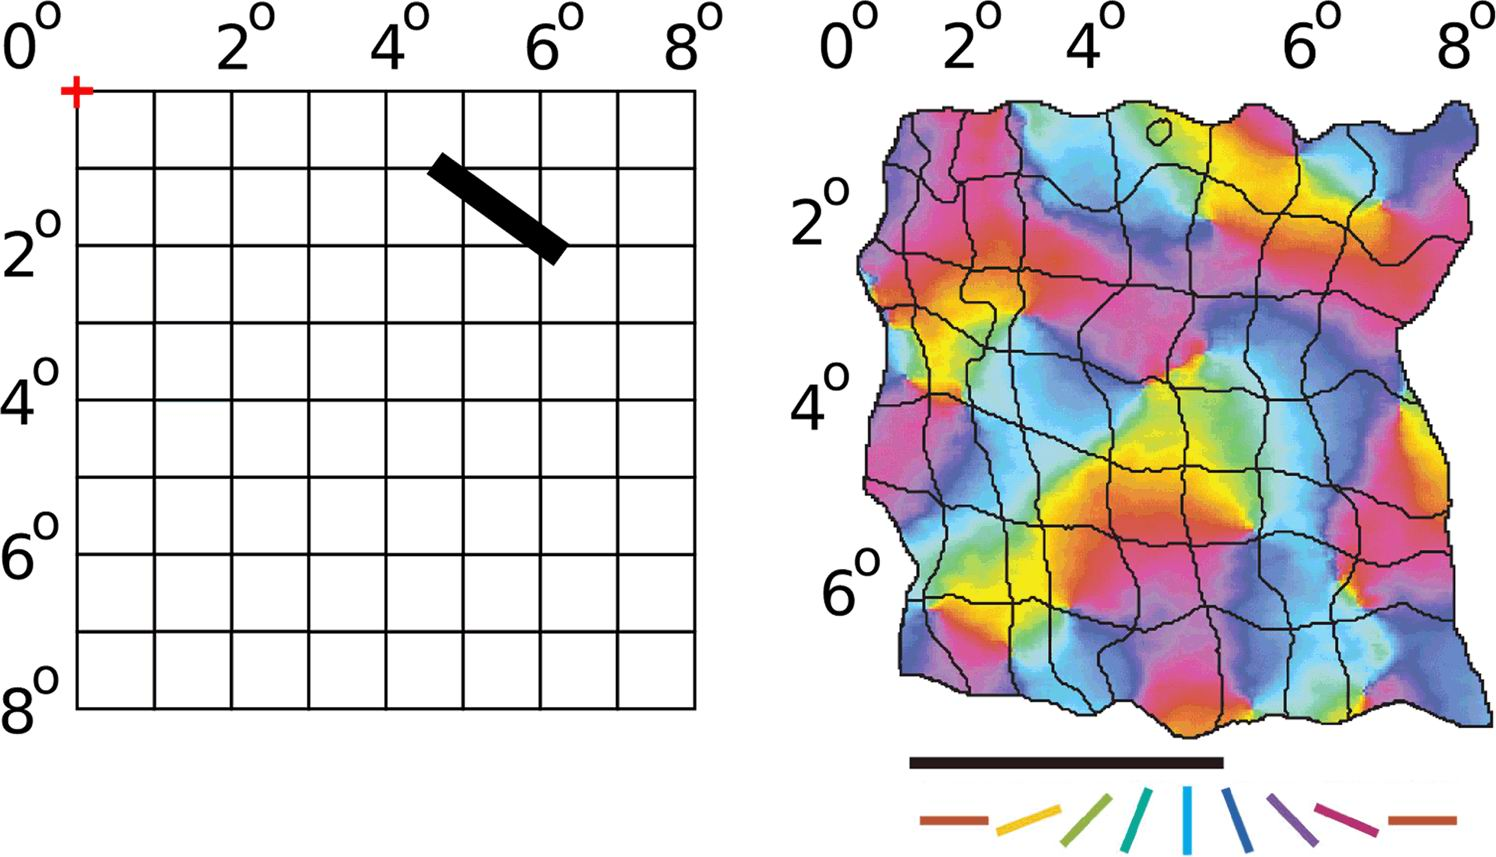
\includegraphics[width=0.8\textwidth]{pics/retinotopic.jpg}
	\caption{The retinotopic and orientation map on the surface of V1 of a tree shrew~\cite{bednar2009topographica}.
	The visual field (left) with a fixation point marked as a red cross on the up-left corner can be divided into a regular grid.
	Each square represents a 1$^\circ \times 1^\circ$ area of visual space.
	In cortical area V1 of mammals, neurons are arranged into a retinotopic map (right) responding to the retinal visual space.
	As an example, the retinotopic map shows the orientation preference of the V1 neurons of a tree shrew for an 8$^\circ \times 7^\circ$ area of visual space (adapted from~\cite{bosking2002spatial}; scale bar is 1 mm).}
	\label{Fig:retinotopic}
\end{figure}

In the spatial domain, V1 neurons are tuned to Gabor-like transforms applied to their small local receptive field.
The retinotopic and orientation map on the surface of V1 of a tree shrew is shown in Figure~\ref{Fig:retinotopic}.
A black bar presented in the retinal image evokes a response in the corresponding grid square of V1 (6$^\circ$, 2$^\circ$) depending on the orientation of the stimulus.
The coloured map on the right represents the preferred orientation of neurons in each location.
Thus the black bar shown at left will activate V1 neurons coloured in purple in the specific square.
In theory, these Gabor-like filters together can carry out neuronal processing of spatial frequency, orientation, motion, direction, speed, and many other spatiotemporal features.
Similar maps could be plotted for this same area showing preference for other visual features.

\subsubsection{Prestriate Cortex: V2}
Visual area V2, also called prestriate cortex~\cite{an2012distinct}, is the second major area located in the occipital lobe of the primate brain, and the first region within the visual association area~\cite{wu2011early}. 
It receives strong feed-forward connections from V1 and has many properties in common with V1. 

The responses of V2 neurons are tuned to simple shapes such as orientation and sinusoidal gratings. 
Moreover, V2 neurons are able to represent variety of higher order shapes that are based on contours (e.g., angles and curves with multiple orientations at different subregions within a single receptive field) or grating patterns~\cite{hegde2000selectivity}.
The responses of many V2 neurons are also modulated for complex properties: orientation of illusory contours~\cite{anzai2007neurons}, binocular disparity~\cite{daniel2009whither}, and whether the stimulus is part of the figure or the ground~\cite{qiu2005figure}.

%In a recent study, the Layer 6 cells of the V2 cortex were found to play a very important role in the storage of Object Recognition Memory as well as the conversion of short-term object memories into long-term memories.[23]

\subsubsection{Visual Area V4}
Area V4 is the third cortical area in the ventral stream, receiving strong feedforward input from V2 and transmitting to the PIT.
It also receives direct inputs from V1 which are mostly generated in the visual central space.
V4 is the first area in the ventral stream to show strong attentional modulation.
Most studies indicate that selective attention can change firing rates in V4 by about 20\%~\cite{filipe2013human}.
This discovery found by Moran and Desimone~\cite{moran1985selective} was the first report of attention effects anywhere in the visual cortex.

Although V4 is mainly modulated for colour recognition, it is also tuned for orientation and spatial frequency similar to V1.
Comparing to V1, V4 responds to more complex object features with intermediate complexity but is not tuned for complex objects as areas in the inferotemporal cortex are~\cite{williams2007biological}.

\subsubsection{Inferotemporal Cortex: IT}
Inferotemporal Cortex is only found in the temporal lobe in primates including humans. 
It is tuned to a range of object features complexity starting with simpler patterns in the PIT/TEO~\cite{tanaka1991coding};
And the complexity increases along the ventral stream towards AIT/TE where objects are represented and recognised~\cite{dean1976effects}.
The high-order complex features includes the combinations of colour or texture with complicated shapes~\cite{tanaka1991coding}, and body parts such as faces and hands~\cite{gross2008single}.
The distinguishing features of the IT cortex is that the neuronal responses are position and size invariant~\cite{schwartz1983shape,logothetis1995psychophysical}, and also invariant to changes in luminance, texture, and relative motion ~\cite{sary1993cue,perry2014feature}.
It is wide-accepted that the identity-preserving transformation invariance makes IT ideal for representing objects despite changes in the surrounding environment and retinal image.

In the next section, this report will explore the detailed mechanism of object representation in this cortical area.
%PFC
\subsection{Object Representation in IT}
\label{sec:orIT}
%\subsection{Untangling Object Representation}
The neuronal representation in the cortical area of IT is considered to be the spatio-temporal pattern of spikes.
The spiking activities of single neurons and populations are thought to hold the key to encode visual information.
In Section~\ref{sec:SNNintro}, the report will introduce single neuron models and spike coding mechanisms in computational spiking neural networks.

\subsubsection{Single neurons}

\begin{figure}[b!]
	\centering
	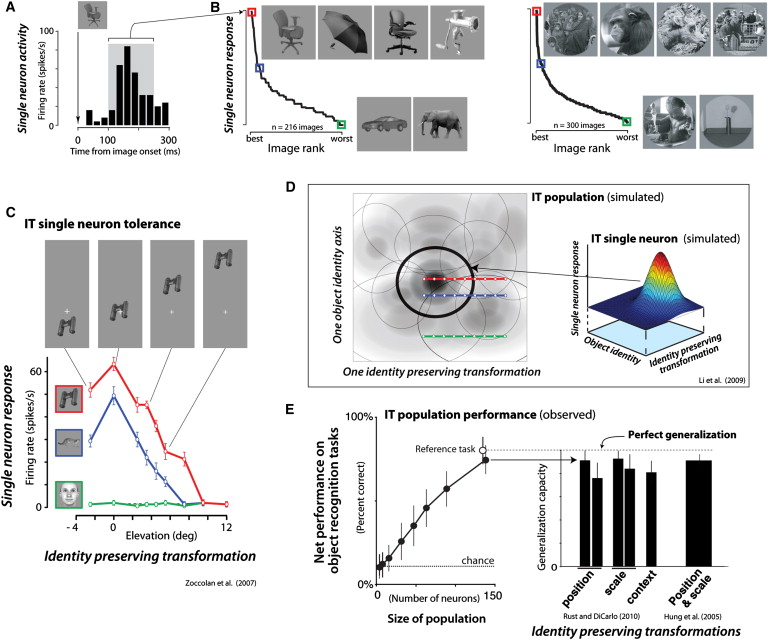
\includegraphics[width=0.9\textwidth]{pics/IT.jpg}
	\caption{	
		IT single-neuron properties and their relationship to population performance~\cite{dicarlo2012does}.
	}
	\label{Fig:IT}
\end{figure}
Most studies have investigated the neural activities in the IT by means of firing rate or spike count.
A typical histogram, Figure~\ref{Fig:IT}(A)~\cite{zoccolan2007trade}, shows the spike count of a single neuron in time bins of 25~ms for a duration of 300~ms in total right after the presentation of a visual image.
The highlighted time window, the so-called `decoding' window, is adjusted to the latency of the conductance along the ventral stream. 
The spike count of the `decoding' window is well modulated for object identity, position or size~\cite{desimone1984stimulus,kaneko1996sequence}, see example in Figure~\ref{Fig:IT}(B) where the left shows the spiking activities for clean figures and the right for natural scenes.
The neural responses were sorted from high to low with the corresponding figures presented, where the red point indicated the highest respond while the green the lowest and the blue the medium.
Another example in Figure~\ref{Fig:IT}(C) shows the responses of an example IT neuron obtained by varying the position (elevation) of three objects with high (red), medium (blue), and low (green) activities.
The object identity preference was maintained in the entire test range regardless of the position changes.
These tuning curves are similar to the well-understood firing rate modulation in visual area V1 on the bar orientation.

%A Contemporary View of IT Single Neurons\\
%Respond to different variations\\
%How do these IT neuronal population phenomena (above)
%depend on the responses of individual IT neurons?
Understanding IT single neuron responses has proven to be extremely challenging and even predicting the responses of an IT neuron to a new image remains impossible.
Nevertheless, IT neurons are activated by complex combinations of visual features and that they are often able to maintain their relative object preference over small to moderate changes in object position, scale, pose~\cite{logothetis1996visual}, illumination~\cite{vogels2002effects} and clutter~\cite{zoccolan2005multiple}.

%respond to more objects\\
Although IT neurons are commonly described as narrowly selective object identifier, neurophysiological studies have shown a diverse selectivity of single neurons~\cite{desimone1984stimulus}.
Most IT neurons are broadly tuned and the typical IT neuron responds to many different images and objects~\cite{zoccolan2007trade}, also see Figure~\ref{Fig:IT}(B).
As illustrated in Figure~\ref{Fig:IT}(D), a single neuron (right) is modulated to both object identities and variables of identity-preserving transformations.
To explain the plot in ~\ref{Fig:IT}(C), position is the variable here; thus the tuning curve for different identities on each position can be described as a slice in the 3-D plot which is Gaussian-like.
As a result, the rank order of the three objects remains the same due to the Gaussian-like curve stays similar.
If a population of such IT neurons tiles with the overlapping fashion, see left panel of Figure~\ref{Fig:IT}(D), a more accurate recognition result containing the transformation parameter can be carried out with population coding.

\subsubsection{Population of neurons}

Spike timing variability in the ms resolution of spikes is consistent with a Poisson-like stochastic spike generation process.
The underlying output rate of IT neurons is determined by each particular image.
Despite the timing variability, the brain can reliably recognise the presented object by integrating the neural responses across IT population~\cite{de2007properties}.
However, it still remains unclear whether the spike timing variability brings down the encoding/decoding accuracy or if it contributes to the population tuning for useful informations~\cite{ermentrout2008reliability}. 

%simple weighted summations of IT spike\\
Although the first stage of the ventral stream, V1, is reasonably well studied, the visual processing in higher stages especially in V4 and IT remains poorly understood.
Nevertheless, as stated above IT is the main part of ventral stream to recognise and categorise the objects in real-time and is tolerant to identity-preserving transformations.
Specifically, simple linear classifier built on the output rates of randomly selected population with only a few hundred neurons reveals a high-level of object recognition performance~\cite{hung2005fast};
and the simple weighted summation explains a wide range of invariant object recognition behaviour sufficiently~\cite{majaj2012unified}.

Figure~\ref{Fig:IT}(E) shows the direct tests of measuring the cross-validated population performance on categorisation tasks using linear classifiers.
The recognition performance approaches ceiling level with only a few hundred neurons (left panel), and the same population shows a good generalization across moderate changes in position, scale, and context.
%50 ms window matters\\
\subsubsection{Decoding Window Matters}
The output spiking pattern of the ventral visual stream are well described by a firing rate code where the decoding window size is 50~ms~\cite{hung2005fast}.
Thus the visual representation in IT is usually found in the first 50~ms of neuronal response, although different time epochs relative to stimulus onset may encode different types of visual information~\cite{brincat2006dynamic} (see Figure~\ref{Fig:IT}(A), an appropriate decoding window can be 100–150~ms after image onset).

%\subsection{IT}




%conclusion\\
%Such findings argue for a distributed representation of visual
%objects in IT, as suggested previously (e.g., Desimone et al.,
%1984; Kiani et al., 2007; Rolls and Tovee, 1995)—a view that
%motivates the population decoding approaches described
%above (Hung et al., 2005; Li et al., 2009; Rust and DiCarlo,
%2010). That is, single IT neurons do not appear to act as sparsely
%active, invariant detectors of specific objects, but, rather, as
%elements of a population that, as a whole, supports object recog-
%nition. This implies that individual neurons do not need to be
%invariant. Instead, the key single-unit property is called neuronal
%‘‘tolerance’’: the ability of each IT neuron to maintain its prefer-
%ences among objects, even if only over a limited transformation
%range (e.g., position changes; see Figure 4C; Li et al., 2009).
%Mathematically, tolerance amounts to separable single-unit
%response surfaces for object shape and other object variables
%such as position and size (Brincat and Connor, 2004; Ito et al.,
%1995; Li et al., 2009; Tove ́e et al., 1994; see Figure 4D). This
%contemporary view, that neuronal tolerance is the required and
%observed single-unit phenomenology, has also been shown for
%less intuitive identity-preserving transformations such as the
%addition of clutter (Li et al., 2009; Zoccolan et al., 2005).


%Summery\\
%Taken together, the neurophysiological evidence can be
%summarized as follows. First, spike counts in 50 ms IT decod-
%ing windows convey information about visual object identity.
%Second, this information is available in the IT population begin-
%ning 100 ms after image presentation (see Figure 4A). Third,
%the IT neuronal representation of a given object across changes
%in position, scale, and presence of limited clutter is untangled
%from the representations of other objects, and object identity can
%be easily decoded using simple weighted summation codes (see
%Figures 2B, 4D, and 4E). Fourth, these codes are readily
%observed in passively viewing subjects, and for objects that
%have not been explicitly trained (Hung et al., 2005). 

In sum, the output of the ventral stream is reflexively expressed in neuronal firing rates across a short interval of 50 ms and is an explicit object representation;
and the rapid production of this representation is consistent with a largely feed-forward, non-linear processing of the visual input~\cite{dicarlo2012does}, which is described in the following section.
\subsection{Hierarchical Feed-forward Organisation }
%Feed-forward, hierarchical organisation and abstraction.

\begin{figure}[h!]
	\centering
	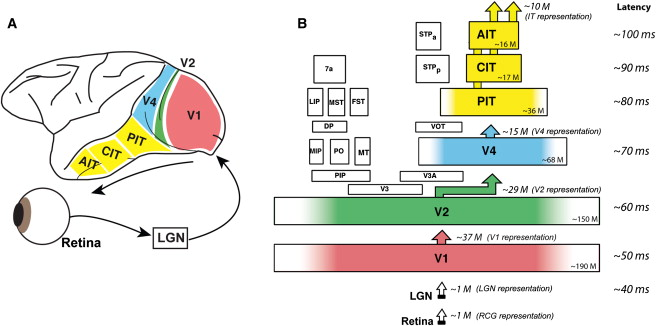
\includegraphics[width=0.9\textwidth]{pics/ventral.jpg}
	\caption{The ventral visual pathway and its hierarchical organization~\cite{dicarlo2012does}.
}
	\label{Fig:Ventral}
\end{figure}
Figure~\ref{Fig:Ventral}(A) illustrates the ventral stream cortical area locations in the macaque monkey brain, and the flow of visual information from the retina.
The corresponding hierarchical organisation is showed in Figure~\ref{Fig:Ventral}(B).
Each area is plotted with the size proportional to its cortical surface size.
Approximate total number of neurons of both hemispheres is shown in the corner of the cortical areas.
The approximate number of projections is written above each block.
In addition, the colour dedicates to processing the central 10$^\circ$ of the visual field.
At last, approximate median response latency is listed on the right.
%of the ventral stream with spikes travelling first from the retina to the lateral geniculate nucleus of the thalamus (LGN), and then through cortical areas introduced above: V1 , V2, V4 to IT. 
\subsubsection{Latency}
Each cortical area along the ventral stream contributes a conductance latency of about 10~ms of the visual information~\cite{nowak1997timing}.
Thus, just around 100~ms after images appeared in front of the retina, a first wave of object identity neuronal activity is present throughout much of IT (e.g., Figure~\ref{Fig:IT}(A)).

\subsubsection{Neurons and Connections}
Because retinal and LGN receptive fields are point-wise spatial sensors, the object visual information conveyed to V1 are nearly as raw as the pixel representation (1 million pixels). 
As V1 carries out its visual process, the total object representation increases approximately 30-times~\cite{stevens2001evolutionary} because of its non-linear filtering.
This dimensionality expansion results in an overcomplete population re-representation~\cite{lewicki2000learning} in which the object representation vectors have more dimensions than the LGN input.
As a result, simulations show that a V1-like representation is clearly better than RGN-like/pixel-based representation, but still far below human performance for real-world recognition problems~\cite{dicarlo2007untangling}.

The output projections of each area decreases from V2 (about 29 million) to AIT which represents the object with 10 million dimensions.
At the same time, the receptive field size of neurons increases to complete the object representation with a whole image and to perform invariant recognition.

%\begin{figure}
%	\centering
%	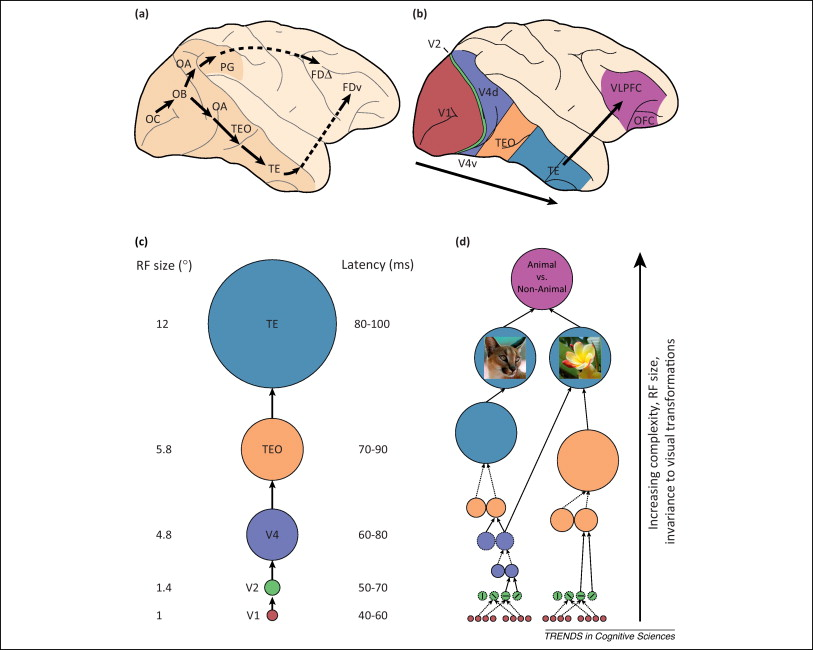
\includegraphics[width=0.9\textwidth]{pics/hierarchi.jpg}
%	\caption{Receptive field sizes of the sub areas along the hierarchical visual processing pathway~\cite{kravitz2013ventral}.}
%	\label{Fig:Hir1}
%\end{figure}
\subsubsection{Tuned Features and Receptive Fields }
\begin{figure}[h!]
	\centering
	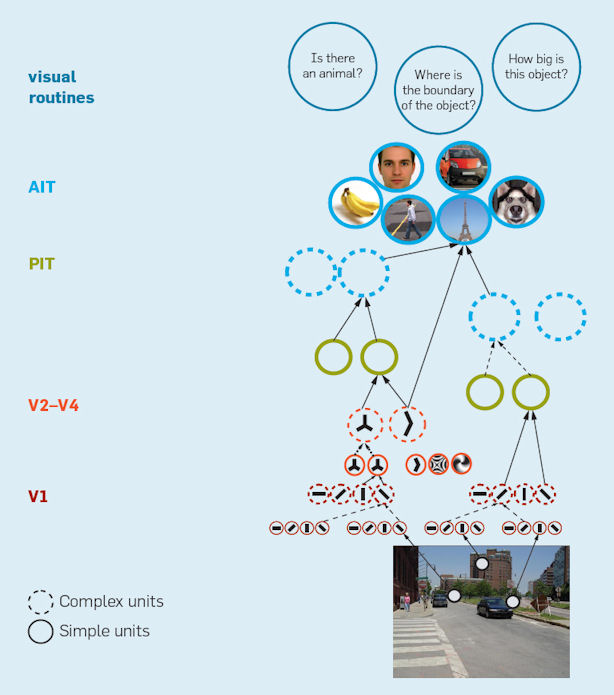
\includegraphics[width=0.9\textwidth]{pics/serre.jpg}
	\caption{The hierarchical ventral stream and the corresponding tuned features for each layer~\cite{serre2010neuromorphic}.}
	\label{Fig:serre}
\end{figure}
As the visual information conducts along the ventral stream, neurons become selective for stimuli that are increasingly complex from simple oriented bars and edges in early visual area V1 to moderately complex features in intermediate areas: V2, V4 and PIT to complex objects and faces in AIT, see Figure~\ref{Fig:serre}.
Along with this growing complexity of the preferred stimulus, the invariance properties of neurons also increase.
Neurons become more and more tolerant with respect to the exact position and scale of the stimulus within their receptive fields.
As a result, the receptive field size of neurons increases from
about one degree or less in V1 to several degrees in IT, see Figure~\ref{Fig:Hir1}.

\begin{figure}[h!]
	\centering
	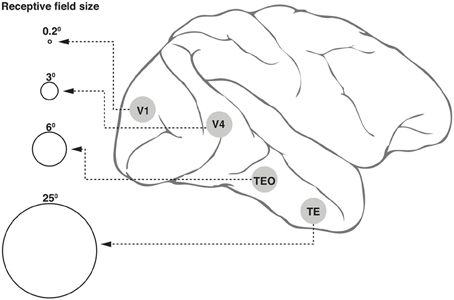
\includegraphics[width=0.9\textwidth]{pics/rf.jpg}
	\caption{Receptive field (RF) sizes along the ventral cortical stream in the primate. While the degree of complexity of processing may increase, the RF size at any one eccentricity also increases dramatically along the various cortical areas from V1 into the temporal pole. The circles shown in the figure are not drawn to scale, but the numbers above the circles indicate approximate relative sizes of the RF diameters.~\cite{vidyasagar2013reading}.}
	\label{Fig:Hir1}
\end{figure}

%\subsubsection{Tuned Features}
%
%V1 are orientation selective for multiple stimulus types, i.e., edges, bars, gratings (Hubel and Wiesel, 1968; Hubel et al., 1978).
%V2 cells encode border ownership (Zhou et al., 2000) which is the first stage of assigning an oriented edge to an object representation.
%Thus contour-based object representation starts in V2.
%Form processing in V4 combines multiple, spatially-adjacent, orientation responses seen in V1 and V2 to encode angles and curvatures (Pasupathy and Connor, 1999).
%These responses advance the nascent object representation from border ownership (Orban, 2008) to responses that are dependent on the placement of the curvature with respect to the center of the shape (Pasupathy and Connor, 2001).
%
%Inferior temporal (IT) cortex has a range of object property complexity starting with simpler features posteriorly (PIT or TEO: Tanaka et al., 1991; Kobatake and Tanaka, 1994) that increase in complexity as processing moves anteriorly (AIT or TE) to represent objects and perform object recognition (Cowey and Weiskrantz, 1967; Gross et al., 1971, 1972; Dean, 1976).
%This includes complex shapes, combinations of color or texture with shape (Gross et al., 1972; Desimone et al., 1984; Tanaka et al., 1991), and body parts (faces or hands: see Gross, 2008 for a review). 
%In addition, responses in IT cortex are position and size invariant (Sato et al., 1980; Schwartz et al., 1983; Rolls and Baylis, 1986; Ito et al., 1995; Logothetis and Pauls, 1995) and also invariant to changes in luminance, texture, and relative motion (Sáry et al., 1993).
%Combined, these characteristics make IT ideal for representing objects despite changes in the surrounding environment and retinal image.

%
%\begin{figure}
%	\centering
%	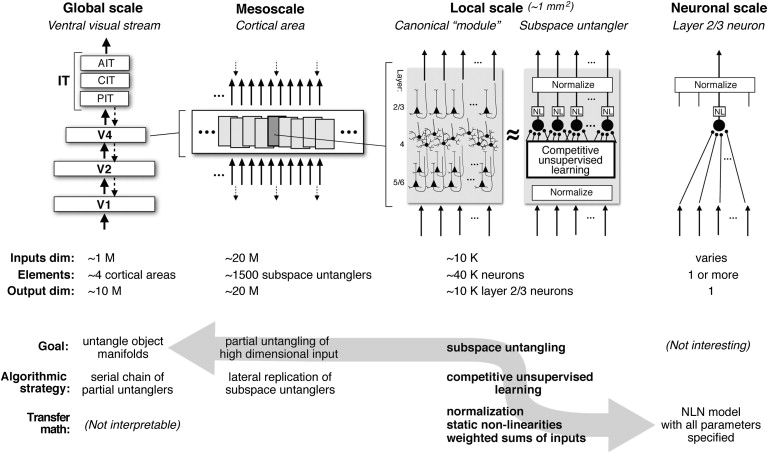
\includegraphics[width=0.9\textwidth]{pics/hierarchiNLN.jpg}
%	\caption{The ventral visual pathway and its hierarchical organization~\cite{dicarlo2012does}.}
%	\label{Fig:HirNLN}
%\end{figure}

\section{Spiking Neural Network}
\label{sec:SNNintro}
The so-called third generation of neural networks~\cite{maass1997networks} introduces a different set of functions and parameters to model neurons;
these both model biological neurons more precisely~\cite{hodgkin1952quantitative} and increase the computational power of networks of neurons if compared to classical sigmoidal units.
Such networks rely on the propagation of an all-or-none signal, the action potential, which asynchronously carries information to its connected units by means of its timing.
\subsection{Neuronal Model}
The level of biological detail of such models varies greatly but many models build on the `leaky integrate and fire' (LIF) model.
Spikes arriving at a LIF neuron cause a temporary flow of current into or out of the neuron, modelling the behaviour of synapses in biological neurons.
The LIF neuron integrates this current over time, accumulating charge which gradually leaks away. If the charge in the neuron reaches a certain threshold, the neuron produces a spike and its charge is reset. 
%\subsubsection{The Membrane Potential}
%A typical neuron is divided into three parts: the dendrites, the soma and the axon. Generally speaking, the dendrites receive the input signals from the previous neurons. The soma is where the received input signals are being processed and the axon is where the output signals are transmitted. The synapse is between every two neurons; if a neuron j sends a signal across the synapse to neuron i, the neuron that sends the signal is called presynaptic and the neuron that receives the signal is called postsynaptic neuron. 
%Hodgkin and Huxley \cite{hhmodel} found out, by experimenting on the squid giant axon, that it is the time of the spikes that encodes information \cite{pnn}, Figure~\ref{dendrites}.
% 
%%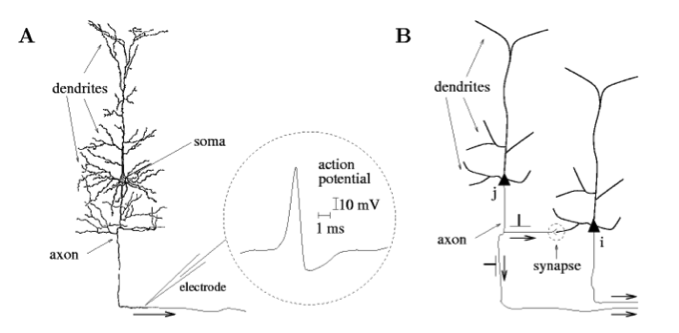
\includegraphics{chapter2/dendrites.png}
%
%\begin{figure}[h!]
%  \centering
%    \centering
%      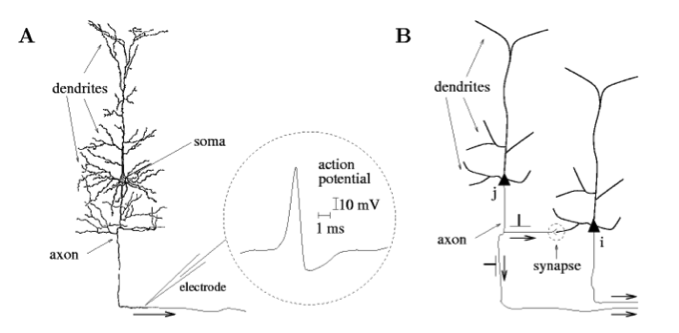
\includegraphics[width=0.5\textwidth]{chapter2/dendrites.png}
%  	\caption{A. The inset shows an example of a neuronal action 
%		potential. 	The action potential is a short voltage pulse of 
%		1-2ms duration and 100mV of amplituted. B. Signal 
%		transmition from a presynaptic neuron j to a post synaptic 
%		neuron i. The synapse is marked by a dashed circle \cite{gernstbook}.}
%	\label{dendrites}
%\end{figure}
%
%A living neuron maintains a voltage drop across its membrane. Every cell is surrounded by positive and negative ions. The main ions are K$^{\textrm{+}}$ (Potassium), Cl$^{\textrm{-}}$ (chloride), Na$^{\textrm{+}}$ (sodium) and Ca$^{\textrm{2+}}$ (calcium). In the inner surface of the membrane there is an excess of negative charges and on the outer surface there is an excess of positive charges. Those charges create the membrane potential.
%
%The membrane potential can be calculated from the following equation: Vm=Vin-Vout, where Vin is the negative charges on the inside of the cell and Vout are the positive charges outside of the cell.  When the membrane potential is at the resting state, that is when it is not receiving any input signals, the resting potential Vrest is set to Vin, which is around -60mV to -70mV.
%
%When the neuron receives an input, some of the ion channels of the cell open and others close, resulting in an electrical current flow into the cell, which results in a change of the resting potential Vrest \cite{princNeuron}.
%
%The phenomenon during which the membrane's potential changes exceed the resting potential is called depolarization. The opposite phenomenon is called hyperpolarization. When the depolarization reaches a critical value, also known as threshold, the cell produces an action potential (a spike) \cite{princNeuron}, figure 1.2. If the membrane potential receives an input that causes depolarization or hyperpolarization and after that does not receive any other input, the membrane potential returns slowly to its resting potential.
%
%In the case of the Glial cell the potassium K+ are flowing from the inside of the cell to the outside causing a potential difference called equilibrium potential Ek \cite{princNeuron} . This E$_{\textrm{k}}$ determines the resting membrane potential and can be calculated from the Nerst Equation:
%
%
%\begin{equation} \label{eq:EK}
%	E_k = {RT \over zF} ln {[X]_o \over [X]_i}
%\end{equation}
% 
%Where R is the gas constant, T is the temperature in Kelvin, z is the valence of the ion, F the Faraday constant, [X]$_{\textrm{o}}$ and [X]$_{\textrm{i}}$ are the concentrations of the ion outside and inside of the cell \cite{princNeuron}.  Thus the Vrest for the Glial cell is Vrest = -75mV. The membrane potential will be discussed in the next section when the Hodgkin-Huxley neuron model will be described based on the experiments on the squid giant axon.
%
%\subsubsection{The Action Potential}
%
%As stated before, when the membrane potential reaches a critical value called threshold it emits an action potential, also known as a spike. This is caused by the movement of ions across the membrane through voltage-gated channels \cite{princNeuron}.  The spikes are identical to each other and their form does not change as the signal moves from a presynaptic to a postsynaptic neuron \cite{gernstbook}. The firing times of a neuron are called spike train and it is represented with the following equation: 
%
%\begin{equation} \label{eq:spiketrain}
%	Fi=\{t^1_i, t^2_i, ..., t^n_i\}
%\end{equation}
%
%The subscript i defines the neuron and the superscript defines the number of the emitted spikes, where n is the most recent emitted spike.
%
%	Directly after the transmission of a spike, the membrane potential goes through a phase of high hyperpolarization under the resting potential and then slowly returns back to the resting potential. During that time, it is not possible to emit a second spike even for strong input signals, that is because the ion channels are open instantly after a spike has been generated \cite{gernstbook}. The minimum time between two generated spikes is called absolute refractory period and the phenomenon where the membrane potential undershoots below the resting potential is known as the spike after potential (SAP), Figure~\ref{sap}.
%
%\begin{figure}[h!]
%  \centering
%    \centering
%      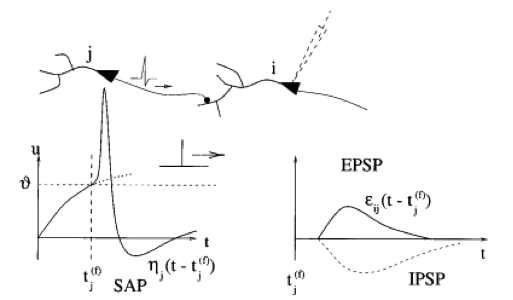
\includegraphics[width=0.5\textwidth]{chapter2/sap.png}
%  	\caption{The membrane potential is increased and at time tj(f) the membrane potential reaches the threshold so a spike is emmited \cite{pnn}.}
%	\label{sap}
%\end{figure}
% 
% \subsubsection{The Synapse}
%
%Between the axon of the presynaptic neuron and the dendrite of the postsynaptic neuron there is a small gap, also known as synaptic gap. The operation of the synapse is very complicated and a detailed description is beyond the scope of this review.
% The spike of the presynaptic neuron cannot cross this gap, however, when a spike arrives from the presynaptic neuron to the synapse the gap is filled a fluid that generates a postsynaptic potential (PSP) to the dendrite of the postsynaptic neuron \cite{princNeuron}. This process does not happen instantaneous; there is a small delay generated in that particular synapse.
% 
%There are two types of postsynaptic potentials. If the generated postsynaptic potential is positive it is called excitatory postsynaptic potential (EPSP) or if the generated postsynaptic potential is negative it is call inhibitory postsynaptic potential (IPSP), Figure~\ref{psp}. An IPSP lowers the membrane potential of the postsynaptic neuron while an EPSP increases it and may cause it to fire a spike.  
%
%\begin{figure}[h!]
%	\centering
%	\centering
%	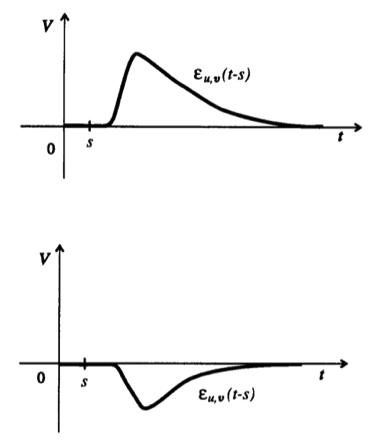
\includegraphics[width=0.3\textwidth]{chapter2/psp.png}
%		\caption{Excitatory postsynaptic potential (EPSP) and Inhibitory 
%			postsynaptic potential (IPSP) of a biological neuron \cite{Maass97networksof}.}
%		\label{psp}
%\end{figure}
%
%\subsubsection{Spiking Neuron Models}
%
%Spiking neuron models can be divided into two major categories \cite{gernstbook} based on their level of abstraction: The conductance models and the threshold models. The conductance models simulate the ion channels of the cell, while the threshold models represent a higher level of abstraction where the threshold voltage has a fixed value and the neuron fires every time the membrane potential reaches it.
%
%	There are two additional models that will not be described in this thesis: the compartmental and rate models. The compartmental models will not be discussed due to their complexity and the rate models are actually the sigmoidal neurons that are used in the traditional artificial neural networks of the 2nd generation. Due to their nature, they neglect all the temporal information of the spikes and only describe their activity as spike rates.
%
%In general, Conductance-Based models have been derived from the Nobel prize winners (1963) Hodgkin and Huxley, based on the experiments that they performed on the giant axon squid \cite{hhmodel}. Basically, they describe what happens to the ion channels of the neuron cell. 
%
%\subsubsection{Leaky-Integrate-and-Fire Model}
%%%%%%%%
%% LIF MODEL START
%%%%%%%%
%
%The Leaky Integrate-and-Fire neurons are threshold-fire models that are based on the summation of all contributions of the presynaptic neurons to the membrane potential. If the membrane potential reaches a fixed threshold from below, the neuron will fire and after an axonal delay it will cause neurotransmitter release from the synapses. 
%
%They have been extensively used in large spiking neural networks \cite{Delorme1999989} because of their ease of implementation and the low computational cost.
%
%The basic circuit of the integrate-and-fire model can be seen in Figure~\ref{lif1new}. It consists of a resistor R in parallel with a capacitor C that models the passive patch of the membrane. In addition, a reset mechanism has been added, as a switch that closes when the membrance potential reaches a threshold value from below. 
%% A pulse coming from a presynaptic neuron, passes from a low-pass RC filter before it is fed to the postsynaptic neuron. 
%
%\begin{figure}[h!]
%\centering
%\centering
%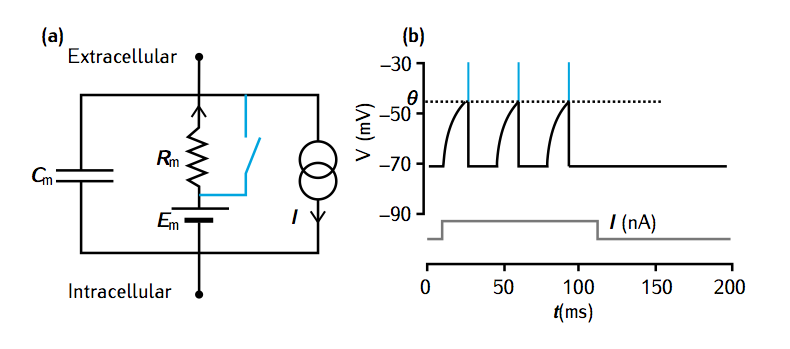
\includegraphics[width=0.7\textwidth]{chapter2/lif1new.png}
%	\caption{The Leaky Integrate-and-fire model. (a) The RC circuit diagram of the model. When the membrane potential reaches a threshold voltage ${\theta}$, the neuron is considered to have fired a spike and the switch closes. The aforementioned short-circuit causes the membrane potential to return back to the resting membrane potential E$_{m}$. (b) Response of LIF circuit to current injection. The refractory period can be observed directly after the firing of a spike \cite{sterratt2011principles}.}
%	\label{lif1new}
%\end{figure}
%
%Using the Ohm's law, the schematic in the Figure~\ref{lif1new} can be described by the following equation:
%
%\begin{equation} \label{eq:lif1}
%C_{m} {dV\over dt} =- { {V - E_{m}} \over R_{m}} + I 
%\end{equation}
%
%Where C$_{m}$ is the membrance capacitance, R$_{m}$ is the membrane reistance and I is the total current flowing into the cell, which could be from an electrode or from other synapses, see equation \ref{eq:neurotrans}. Furthermore, by setting ${\tau}_{m}$ = RC, the equation \ref{eq:lif1} could be rewritten as:
%
%\begin{equation} \label{eq:lif2}
%{\tau}_{m} {dV\over dt} = -V + E_{m} + R_{m}I
%\end{equation}
%
%Where ${\tau}_{m}$ is known as membrane time constant. When the membrane potential reaches a predefined threshold ${\theta}$, the neuron fires a spike and the membrane potential is reset to E$_{m}$.\\
%
%The electrical current resulting from the neurotransmitter at time t$_{s}$ is, for t >= t$_{s}$:
%
%\begin{equation} \label{eq:neurotrans}
%	I_{syn}(t) = g_{syn}(t)(V(t) - E_{syn})
%\end{equation}
%
%Where g$_{syn}$(t) is the synaptic conductance which peaks at $\bar{g}_{syn}$, V(t) is the membrane voltage of the postsynaptic neuron, for conductance-based synapses (COBA) and E$_{syn}$ is the reversal potential of the synaptic conductance. In many cases equation \ref{eq:neurotrans} can be simplified so that synapses can be thought of as sources of current instead of conductance (CUBA), this is done by setting V = V$_{rest}$ in equation \ref{eq:neurotrans}. This simplification is a good approximation for excitatory synapses but not for inhibitory synapses where the inhibitory reversal potential could be close or even above the resting potential \cite{Schutter:2009:CMM:1822639}. The three commonly used equations for the synaptic conductance are the: (a) single exponential decay, (b) alpha function and (c) dual exponential function:
%
%%\begin{subequations}
%%\label{eq:synapsess}
%%\begin{gather*}
% % g_{syn}(t) = \bar{g}_{syn} exp(-{{t-t_{s}}\over \tau})  \label{singleexp} \\
%  %g_{syn}(t) = \bar{g}_{syn} {{t-t_{s}}\over \tau } exp(-{{t-t_{s}}\over \tau})  \label{alfafunc} \\
%  %g_{syn}(t) = \bar{g}_{syn} {{\tau_{1}  \tau_{2} }\over {\tau_{1} - \tau_{2} } }   (exp(-{{t-t_{s}}\over \tau_{1} }) - exp(-{{t-t_{s}}\over \tau_{2} })  \label{dualexp}
%%\end{gather*} 
%%\end{subequations}
%
%\begin{subequations}
%\label{eq:synapsess}
%\begin{align}
%  g_{syn} &= \bar{g}_{syn} exp(-{{t-t_{s}}\over \tau})  \label{singleexp} \\
%  g_{syn} &= \bar{g}_{syn} {{t-t_{s}}\over \tau } exp(-{{t-t_{s}}\over \tau})  \label{alfafunc} \\
%  g_{syn} &= \bar{g}_{syn} {{\tau_{1}  \tau_{2} }\over {\tau_{1} - \tau_{2} } }   (exp(-{{t-t_{s}}\over \tau_{1} }) - exp(-{{t-t_{s}}\over \tau_{2} })  \label{dualexp}
%\end{align} 
%\end{subequations}
%
%Finally, a number of variations of the Leaky Integrate-and-Fire have been proposed to model more complex firing patterns such as the firing rate adaptation or bursting (Type II firing). These models are the Quadratic Integrate-and-Fire model and the Exponential Integrate-and-Fire-model \cite{sterratt2011principles}.

%Section~\ref{sec:np} of this paper presents the details of the hardware of the proposed neuromorphic system, including the silicon retina and the SpiNNaker platform.
%The neural network models are defined and tested on Matlab, and the model structures and experimental results stated in Section~\ref{sec:cnn}.
%In Section~\ref{sec:rrs}, the rate-based models are converted into spiking neurons, and real-time live recognition and recorded data experiments are carried out.
%The contribution of this work is summarised and the future directions are provided in Section~\ref{sec:cfw}.
%\subsection{Spike Coding}
%Dynamic recognition takes advantage of the intrinsic temporal processing of SNNs which are receiving considerable attention for  undertaking vision processing.
%Pattern information can be encoded in the delays between the pre- and post-synaptic spikes since the spiking neurons are capable of computing radial basis functions (RBFs)~\cite{hopfield1995pattern}.
%Spatio-temporal information can also be stored in the exact firing time rather than relative delays~\cite{natschlager1998spatial}.
%Maass~\cite{maass1997networks} has proved mathematically that:
%1) networks of spiking neurons are computationally more powerful than the first and second generation of neural network models;
%2) a concrete biologically relevant function can be computed by a single spiking neuron, replacing  hundreds of hidden units in a sigmoidal neural net;
%3) any function that can be computed by a small sigmoidal neural net can also be computed by a small network of spiking neurons.
%\subsubsection{Rate Coding}
%
%In rate coding the information is encoded into the mean firing rate of the neuron also known as temporal average \cite{gernstbook}:
%
%\begin{equation} \label{eq:lif2}
%v = {{n_{sp}(T)} \over T}
%\end{equation}
%
%Where T is time window, nsp(T) are the number spikes emitted during the time window. There are three averaging procedures \cite{gernstbook}: Rate as a spike count (average over time), rate as a spike density (average over several runs) and rate as a population activity (average over several neurons).
%
%\subsubsection{Temporal Coding}
%
%In temporal coding the information is encoded in the form of spike times \cite{Bohte:2004:ENI:990372.990380}. Hopfield \cite{hopfield_pattern_1995} has proposed a method for encoding analogue data into timing of the spikes with respect to an oscillatory pattern of activity. This method has been proven experimentally in the electric fish. In addition, Maass \cite{Maass97networksof} proposed a method of encoding analogue information in the form of firing times. A different approach has been suggested by Wen and Sendhoff \cite{Jin:2007:EMO:1776814.1776856}, where the input neurons encode information directly into spiking times and an additional bias neuron is used as a time reference. Finally, in polychronization \cite{Izhikevich:2006:PCS:1117652.1117653}, proposed by Izhikevich,  the synaptic delays are tuned so that a neuron would respond to particular spatio-temporal patterns of activity.
%
%\subsubsection{Population Coding}
%
%In population coding a number of input neurons (population) are involved in the analogue encoding and produce different firing times. Bohte et al. \cite{Bohte02unsupervisedclustering} proposed a way of representing analogue input values into spike times using population coding. Multiple Gaussian Receptive Fields (GRF) were used so that the input neurons will encode an input value into spike times, Figure~\ref{codpop1}.  
%
%\begin{figure}[h!]
%\centering
%\centering
%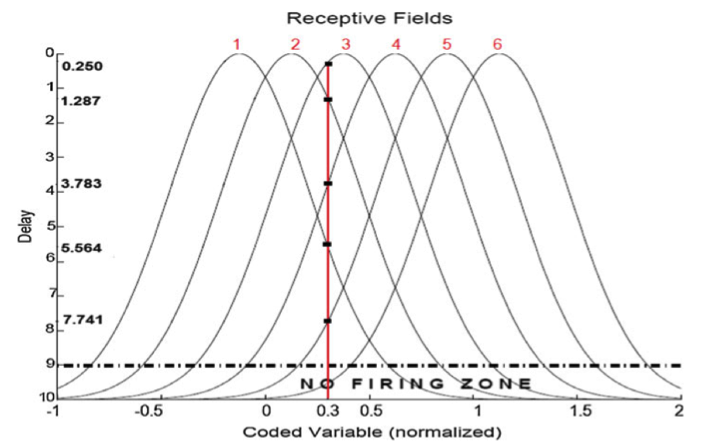
\includegraphics[width=0.7\textwidth]{chapter2/codpop.png}
%	\caption{ Encoding with Gaussian Receptive Fields. The horizontal axis represents the real input data, the vertical axis represent the firing times of the input neurons to an input value 0.3 \cite{Meftah:2010:SED:1873252.1873282}. }
%	\label{codpop1}
%\end{figure}
%
%Firstly the range of the input data has to be calculated. Then the values Imax and Imin, which are the maximum and minimum values of the input data, have to be defined. Furthermore, the number of GRF neurons that are going to be used has to be chosen through the m variable. Lastly, the center of each GRF neuron is calculated from C$_{i}$ while the width of each GRF neuron is calculated by ${\sigma_i}$ \cite{Meftah:2010:SED:1873252.1873282}:
%
%\begin{subequations}
%\label{eq:popcod}
% \begin{align}
%  C_i = I_{min} +{{(2i-3)}\over 2}    {{(I_{max} - I_{min})}\over m-2} \label{ci} \\
%  \sigma_i = {1\over \gamma} {{(I_{max} - I_{min})}\over m-2} \label{si}
% \end{align}
%\end{subequations}
%
%Where ${\gamma}$ is constant number usually around 1.5. A threshold value has to be used so that GRF neurons, that are below the threshold, should not fire.  In the example of Figure~\ref{codpop1} the analogue value 0.3 is encoded into firing times of neuron 3 (0.250ms), neuron 2 (1.287ms), neuron 4 (3.783ms), neuron 1 (5.564ms) and neuron 5 (7.741ms). Neuron 6 does not emit a spike because it's below the threshold. 
%
%A different approach to population encoding was proposed by Eliasmith et al. in \cite{Eliasmith02}, where the firing rates of a heterogeneous population of neurons is used to encode an analogue value. Also, the rank-order coding proposed in \cite{Thorpe2001715} encodes an input value based on the order of spikes of a population.  

\subsection{Learning}
One of the key parameters of a neural network is the amount of influence
each incoming spike has on a neuron. Typically, this influence is modelled
by assigning a `weight' to each synapse which scales the impact of a spike
arriving via that synapse.
Models of many types of learning revolve around modelling changes in
weights over long periods of time observed within the brain. The exact
rules by which these weights are adjusted is the subject of much active
research though most promising approaches attempt to learn from the
relative timing \cite{pfister2006triplets} or rate \cite{bienenstock1982theory} of spikes
arriving at a neuron. As well as adjusting weights, some learning rules
can also form entirely new connections between previously unconnected
neurons \cite{bamford2010synaptic}.
%In 1949 Hebb formulated the famous Hebb law \cite{Hebb1949}: ''When an axon of cell A is near enough to excite cell B or repeatedly or persistently takes part in firing it, some growth process or metabolic change takes place in one or both cells such that A's efficiency, as one of the cells firing B, is increased''.
%
%Hebb's law is modified so that the weights are updated based on the pre and postsynaptic activity of the neurons, also known as Spike Time Dependent Plasticity (STDP) \cite{gernstbook}.
%
%\begin{figure}[h!]
%\centering
%\centering
%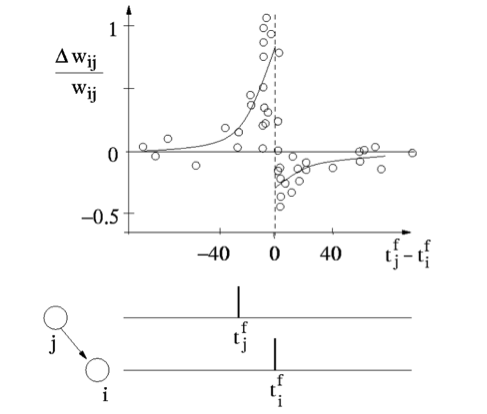
\includegraphics[width=0.7\textwidth]{chapter2/bigpoo.png}
%	\caption{ The weights are changing only if the firing times of neurons j and i are close to each other. Data taken from the experiments of Bi and Poo \cite{bigpoo}. }
%	\label{bigpoo1}
%\end{figure}

%In Figure \ref{bigpoo1} neuron j is the presynaptic neuron, neuron i is the postsynaptic neuron and t$_{j}^{f}$ is the presynaptic fire time and tif is the postsynaptic fire time.
%
%Furthermore, Bi and Poo \cite{bigpoo,bipoo2} found out that the synaptic efficacy $\Delta$w$_{ij}$ is a function of the spike times of the presynaptic and postsynaptic neurons. Hence the term Spike Timing-Dependent Plasticity.
%
%	A way to calculate the synaptic weight updates has been proposed by Gerstner et al. \cite{gernstbook} with the use of exponential learning windows:
%
%\begin{equation}
%  \Delta W = \left\{ 
%  \begin{array}{l l}
%    A_{+}exp(s/\tau_{1}) & \quad \text{if $s$ < 0}\\
%    A_{-}exp(s/\tau_{2}) & \quad \text{if $s$ > 0}\\
%  \end{array} \right.
%\end{equation}
%
%Where s = t$_{j}^{(f)}$-t$_{i}^{(f)}$ is the time difference between presynaptic and postsynaptic firing times. The $\tau_{1}$ and $\tau_{2}$ are constants and the A$_{+}$ and A$_{-}$ are used for stability issues in order to cap the weights to a maximum and minimum value, Figure \ref{dw1}. 
%
%\begin{figure}[h!]
%\centering
%\centering
%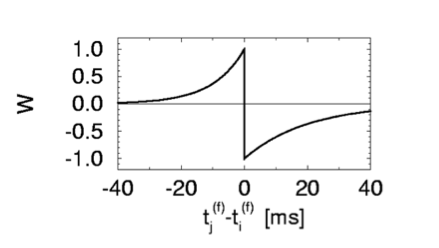
\includegraphics[width=0.4\textwidth]{chapter2/stdpdw.png}
%	\caption{ The exponential learning window as a function the difference between the presynaptic and the postsynaptic firing times. A$_{+}$=1, A$_{-}$=-1, $\tau_{1}$=10ms, $\tau_{2}$=20ms \cite{gernstbook}. }
%	\label{dw1}
%\end{figure}
%
%Numerous methods have been proposed in order to overcome the need of capping the weights to maximum and minimum values for unsupervised learning. For example, the BCM theory, named after the names of the authors ($\bf B$ienenstock, $\bf C$ooper, $\bf M$unro) and it is based on experiments they conducted on neurons in the primary sensory cortex \cite{Bienenstock}. This method uses a sliding threshold mechanism to overcome the saturation of the weights during STDP. However, this method is too computationally expensive thus making it inadequate for large-scale simulations.

\subsection{Successful Applications}
Numerous applications using SNN-based vision processing have been successfully carried out in the past. 
A dual-layer SNN has been trained using Spike Time Dependent Plasticity (STDP) and employed for character recognition~\cite{gupta2007character}. 
Lee et al.~\cite{6467270} have implemented direction selective filters in real time using spiking neurons, considered as a convolution layer in the model of a so called CNN~\cite{camunas2012event}. 
Different features, such as Gabor filter features (scale, orientation and frequency) and shape can be modelled as layers of feature maps. 
The similar behaviours have been found in the primary visual cortex (V1) in the visual pathway~\cite{rehn2007network} as the foundation for higher level visual process e.g. object recognition.
Rank order coding, as an alternative to conventional rate-based coding, treats the first spike as the most important and has been successfully applied to an orientation detection training process~\cite{delorme2001networks}. 
Nengo~\cite{eliasmith2011nengo} is a graphical and scripting based software package for simulating large-scale neural systems and has been used to build the world's largest functional brain model, Spaun~\cite{eliasmith2012large}. 
An FPGA implementation of a Nengo model for digit recognition has been reported~\cite{naylor2013managing}. 
Deep Belief Networks (DBNs), the 4th generation of artificial neural network, have shown great success in solving classification problems. 
Recent study~\cite{o2013real} in this area has mapped an offline-trained DBN onto an efficient event-driven spiking neural network for digit recognition tasks with resounding success.





\section{Platforms}
\label{sec:plt}
The outline of the platform is illustrated in Figure~\ref{fig:SysOverViewa}, where the hardware system is configured, controlled and monitored by the PC.
%Figure~\ref{fig:SysOverViewb} shows the combined hand posture recognition system; 
The jAER~\cite{delbruck2008frame} event-based processing software on the PC configures the retina and displays the output spikes through a USB link.
The host communicates to the SpiNNaker board via Ethernet to set up its runtime parameters and to download the neural network model off-line.
It visualises~\cite{6252490} the spiking activity of the network in real-time.
The photograph of the hardware platform, Figure~\ref{fig:SysOverViewb}, shows that the silicon retina connects to the SpiNNaker 48-node system via a Spartan-6 FPGA board~\cite{galluppi2012real}.
%, which was also applied to a sound localisation system.


\begin{figure}[h!]
\centering
	\begin{subfigure}[t]{0.6\textwidth}
		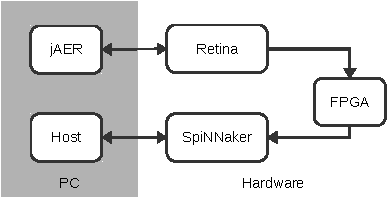
\includegraphics[width=\textwidth]{pics/outline.pdf}
	    \caption{Outline of the platform.}
	    \label{fig:SysOverViewa}
	\end{subfigure}
	\\
	\begin{subfigure}[t]{0.9\textwidth}
		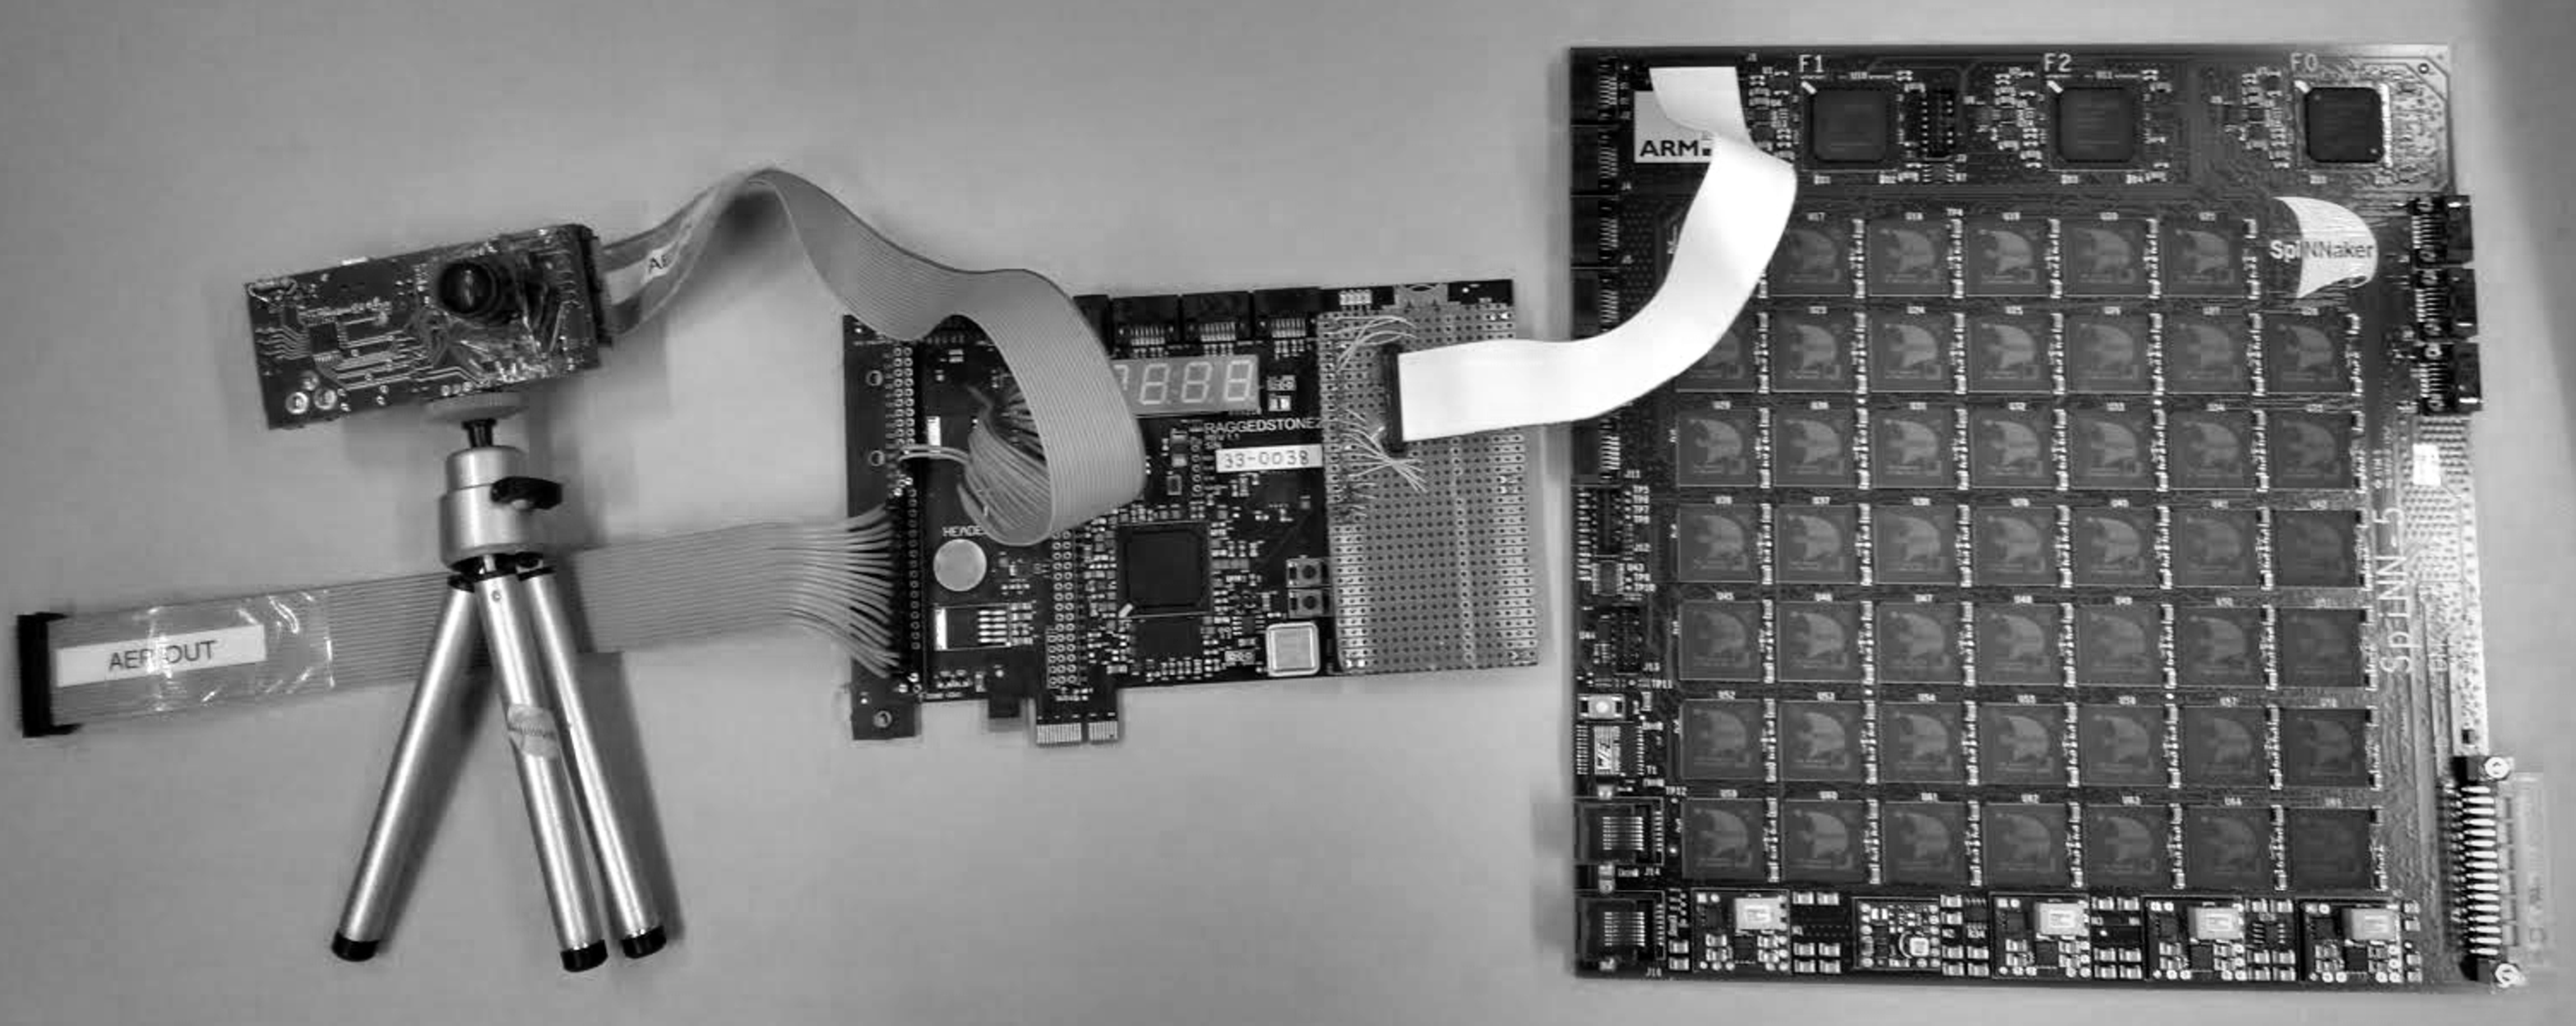
\includegraphics[width=\textwidth]{pics/outline2.pdf}	    \caption{Picture of the hardware platform. From left to right: a silicon retina, a FPGA board, and a 48-node SpiNNaker system.}
	    \label{fig:SysOverViewb}
	\end{subfigure}	

\caption{System overview of the dynamic hand posture recognition platform. 
%The silicon retina connects to the SpiNNaker system through an FPGA board. 
%Spikes from the retina are streamed to the SpiNNaker system through this Spartan-6 FPGA board.
%The jAER software configures the retina and displays its outgoing spikes through the USB connection.
%The host sets up the runtime parameters off-line and downloads the network model to the SpiNNaker system.
}
\label{fig:SysOverView}
\end{figure}


\subsection{Vision Processing Front-ends}
The visual input is captured by a DVS silicon retina, which is quite different from conventional video cameras.
Each pixel generates spikes when its change in brightness reaches a defined threshold.
Thus, instead of buffering video into frames, the activity of pixels is sent out and processed continuously with time.
The communication bandwidth is therefore optimised by sending activity only, which is encoded as pixel events using Address-Event Representation (AER~\cite{lazzaro1995multi}) protocol.
The level of activity depends on the contrast change; pixels generate spikes faster and more frequently when they are subject to more active change.
The sensor is capable of capturing very fast moving objects (e.g., up to 10 K rotations per second), which is equivalent to 100 K conventional frames per second~\cite{lenero20113}.

\subsection{SNNs Back-ends}
The SpiNNaker project's architecture mimics the human brain's biological structure and functionality. 
This offers the possibility of utilizing massive parallelism and redundancy, as the brain, to provide resilience in an environment of unreliability and failure of individual components.

In the human brain, communication between its computing elements, or neurons, is achieved by the transmission of electrical `spikes' along connecting axons. 
The biological processing of the neuron can be modelled by a digital processor and the axon connectivity can be represented by messages, or information packets, transmitted between a large number of processors which emulate the parallel operation of the billions of neurons comprising the brain.

\begin{figure}[h!]
	\centering
	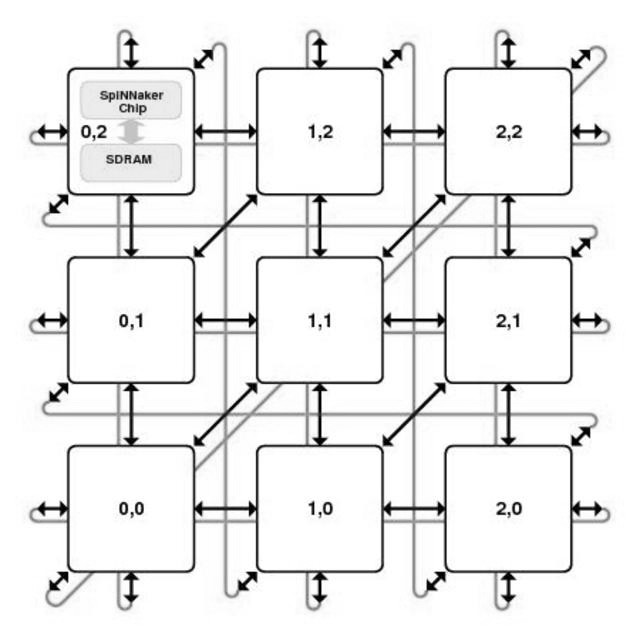
\includegraphics[width=0.85\textwidth]{pics/mesh_ctiff.jpg}
	\caption{SpiNNaker system diagram.
		Each element represents one chip with local memory.
		Every chip connects to its neighbours through the six bi-directional on-board links. }
	\label{fig:sysdia}
\end{figure}

The engineering of the SpiNNaker concept is illustrated in Figure~\ref{fig:sysdia} where the hierarchy of components can be identified. 
Each element of the toroidal interconnection mesh is a multi-core processor known as the `SpiNNaker Chip' comprising 18 processing cores. 
Each core is a complete processing sub-system with local memory.
It is connected to its local peers via a Network-on-Chip (NoC) which provides high bandwidth on-chip communication and to other SpiNNaker chips via links between them. 
In this way massive parallelism extending to thousands or millions of processors is possible.



%The knowledge content and learning ability of the brain is generally thought to be embodied in its evolvable interconnection pattern.
%This structure routes a spike generated by one neuron to others which are interconnected with it via axons and these interconnections are modified and extended as a result of learning processes.
%
%In SpiNNaker a packet router within each multi-core processor controls the neural interconnection. 
%Each transmitted packet represents a spike and simply identifies its source neuron.
%This is used by routers to identify whether a packet should be routed to a processor core, or should be routed on to one of the six adjacent chips connected to it as part of the overall SpiNNaker network.

The `103 machine' is the name given to the 48-node board which we use for the hand posture recognition system, see Figure~\ref{fig:48node}.
It has 864 ARM processor cores, typically deployed as 768 application, 48 monitor and 48 spare cores. 
%The `103 machine' requires a 12V 6A supply. 
%The control interface is via two 100Mbps Ethernet connections, one for the board management processor and the second for the SpiNNaker array. 
%There are options to use the nine on-board 3.0~Gbps high-speed serial interfaces (using SATA cables, but not necessarily the SATA protocol) for I/O; 
%this will require suitable configuration of the on-board FPGAs that provide the high-speed serial interface support. 
The boards can be connected together to form larger systems using high-speed serial interfaces. 

%\begin{figure}
%\centering
%	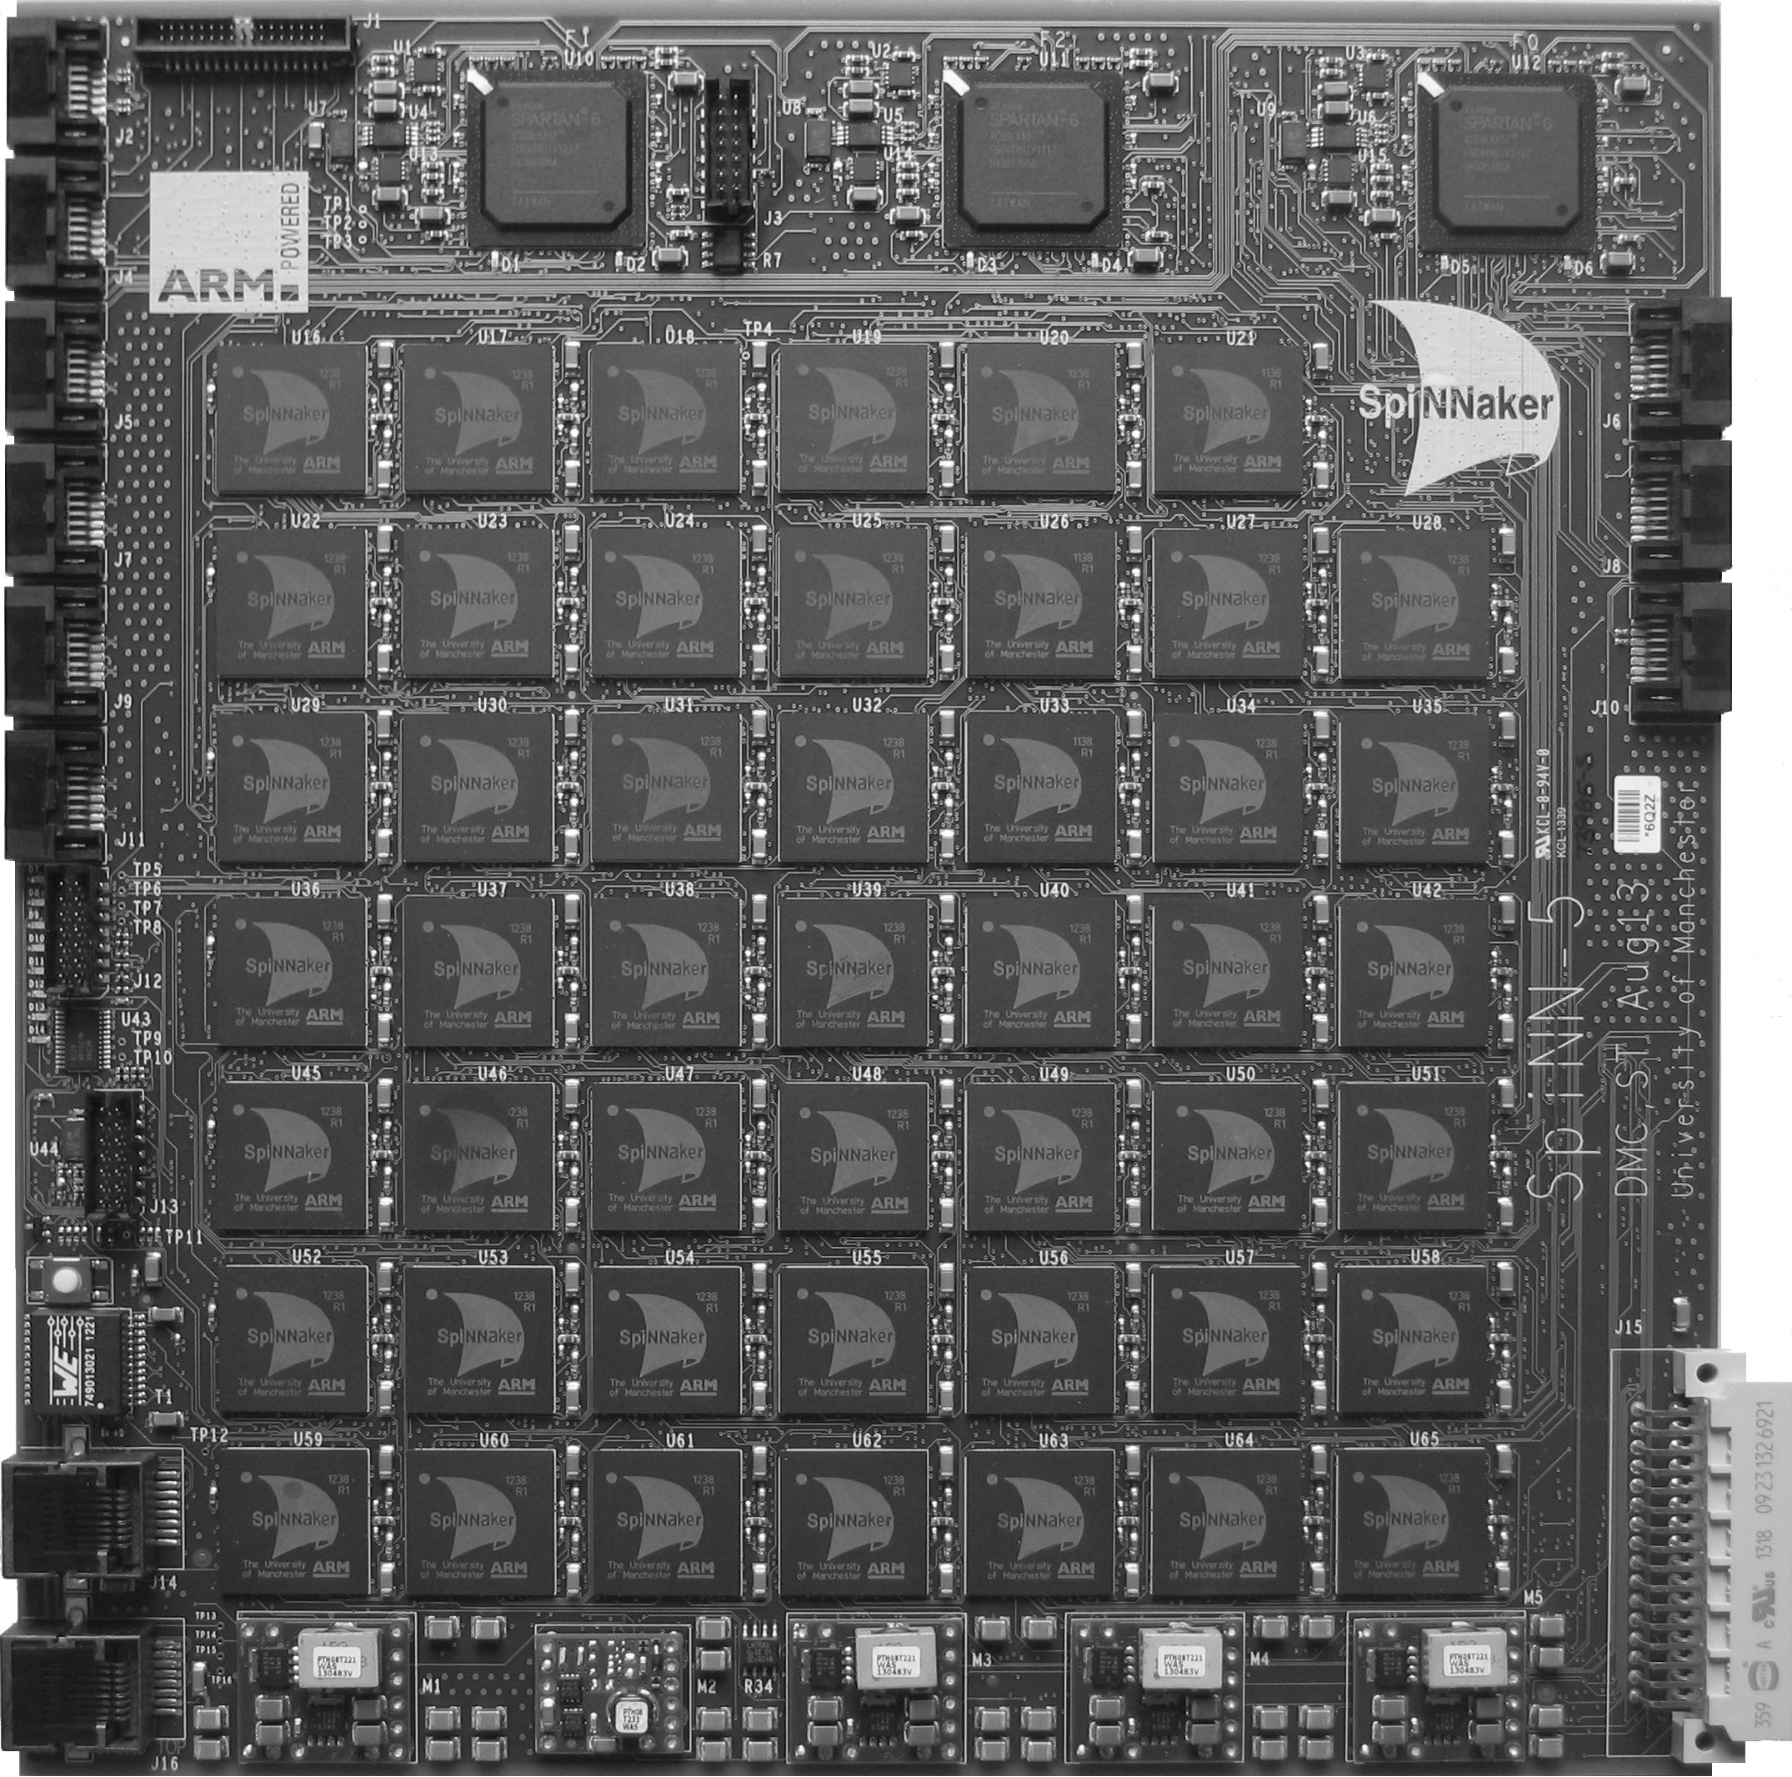
\includegraphics[width=0.6\textwidth]{pics/SpiNN5.pdf}
%	\caption{`103 Machine' PCB}
%	\label{fig:48node}
%\end{figure}

\subsection{SpiNNaker distinguishing features}
Spikes from the silicon retina are injected directly into SpiNNaker via a SPARTAN-6 FPGA board that translates them into a SpiNNaker compatible AER format~\cite{appnote8}. 

From a neural modelling point of view, interfacing the silicon retina is performed using pyNN~\cite{davison2008pynn}. 
The retina is configured as a spike source population that resides on a virtual SpiNNaker chip, to which an AER sensor's spikes are directed, thus abstracting away the hardware details from the user\cite{galluppi2012real}.
Besides the retina, we have successfully connected an AER based silicon cochlea~\cite{5537164} to SpiNNaker for a sound localisation task~\cite{6706931}, see Figure~\ref{fig:sound}.

\begin{figure}[h!]
	\centering
	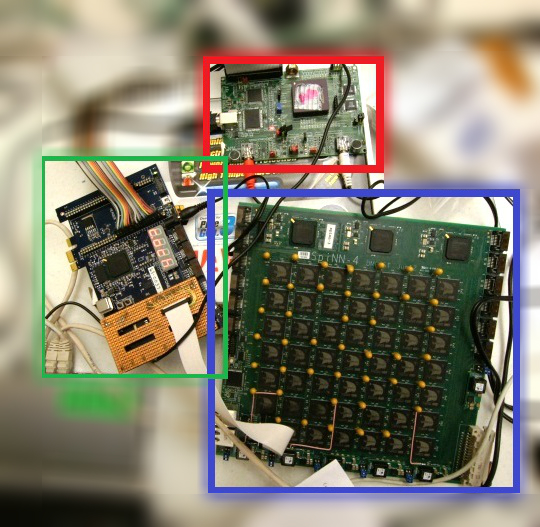
\includegraphics[width=\textwidth]{pics/photooutline_blurred.jpg}
	\caption{Neuromorphic platform for sound localisation: a silicon cochlea connects to a 48-node SpiNNaker board via a FPGA.}
	\label{fig:sound}
\end{figure}

